%==============================================================
%  Póster A0 vertical — CTAP en cadenas SSH  (v2, rediseño)
%  Compilar:  pdflatex poster_v2.tex
%==============================================================
\documentclass[final]{beamer}
\usepackage[size=a0,orientation=portrait,scale=1.38]{beamerposter}
\usetheme{default}
\usepackage[T1]{fontenc}
\usepackage[utf8]{inputenc}
\usepackage{helvet}\renewcommand{\familydefault}{\sfdefault}
\usepackage{graphicx}
\usepackage{amsmath,amssymb,bm}
\usepackage{braket}
\usepackage{qrcode}
\usepackage{booktabs}

\graphicspath{{figures/}}

% --- Paleta refinada ---
\definecolor{navy}{HTML}{12395F}
\definecolor{amber}{HTML}{F2A93B}
\definecolor{coral}{HTML}{D85A30}
\definecolor{tealc}{HTML}{1D9E75}
\definecolor{ptblue}{HTML}{2F7FC9}
\definecolor{darktext}{HTML}{2B2B29}
\definecolor{captiongray}{HTML}{6A6A6A}
\definecolor{bodybg}{HTML}{F5F4F1}

\setbeamertemplate{navigation symbols}{}
\setbeamertemplate{blocks}[rounded][shadow=false]
\setbeamercolor{block title}{fg=white,bg=coral}
\setbeamercolor{block body}{fg=darktext,bg=bodybg}
\setbeamerfont{block title}{size=\large,series=\bfseries}
\setbeamercolor{titlebar}{fg=white,bg=navy}
\setbeamercolor{banner}{fg=darktext,bg=amber}
\setbeamercolor{footer}{fg=white,bg=navy}

\newcommand{\figcap}[1]{\par\vspace{0.22cm}{\small\itshape\color{captiongray}#1}}

% altura exacta de columna = área útil - (cabecera + banner + pie + huecos)
\newlength{\colheight}
\setlength{\colheight}{\dimexpr\textheight-485pt\relax}
% separación mínima entre bloques (el resto lo reparte \vfill)
\newcommand{\blockgap}{\vspace{0.55cm}\vfill}

\begin{document}
\begin{frame}[t]

%==================== CABECERA ====================
\begin{beamercolorbox}[wd=\textwidth,sep=22pt,center,rounded=true]{titlebar}
  {\fontsize{48}{58}\selectfont\bfseries Quantum control for quantum information transfer\\ mediated by topological edge states}\\[10pt]
  {\fontsize{27}{33}\selectfont Miguel García-Mier García \;\textbullet\; MSc in Quantum Technologies \;\textbullet\; UIMP \;\textbullet\; Thesis Supervisor: Gloria Platero\;\textbullet\; Thesis Co-Supervisor: Yue Ban }
\end{beamercolorbox}

\vspace{0.45cm}

\begin{beamercolorbox}[wd=\textwidth,sep=13pt,center,rounded=true]{banner}
  {\fontsize{36}{44}\selectfont\bfseries The control protocol — not topology alone — decides robustness}
\end{beamercolorbox}

\vspace{0.7cm}

%==================== COLUMNAS ====================
\begin{columns}[t,onlytextwidth]

%---------------- COLUMNA 1 : EL PROBLEMA (coral) ----------------
\setbeamercolor{block title}{fg=white,bg=coral}
\setbeamertemplate{itemize item}{\color{coral}\textbullet}
\begin{column}{0.315\textwidth}
\begin{minipage}[t][\colheight][s]{\linewidth}

  \begin{block}{1 · SSH model \& domain walls}
    The SSH chain has alternating hoppings $v$ (intracell) and $w$ (intercell).
    For $v<w$ it is a 1D topological insulator ($\nu=1$) with exponentially
    localized zero-energy edge states protected by \textbf{chiral symmetry};
    bulk gap $\Delta = 2|w-v|$. A \textbf{domain wall} hosts three protected
    states near $E=0$ — $\ket{L},\ket{S},\ket{R}$ — an effective three-site chain:
    \[ H_\mathrm{eff}=J_{LS}\ket{S}\!\bra{L}+J_{SR}\ket{R}\!\bra{S}+\mathrm{H.c.} \]
    \centering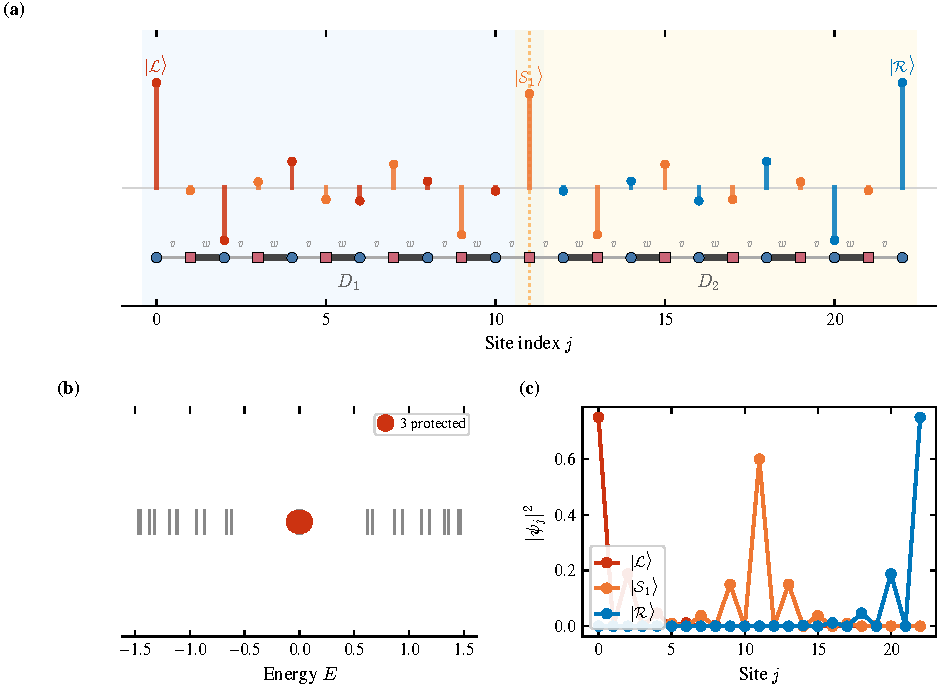
\includegraphics[width=\linewidth]{fig2_domain_wall_states.pdf}
    \figcap{\textbf{Fig.~2} — three protected states in a two-domain SSH chain.}
  \end{block}
  \blockgap

  \begin{block}{2 · Symmetric transfer works}
    An adiabatic ramp of $v(t)$ drives $\ket{L}\!\to\!\ket{S}\!\to\!\ket{R}$.
    Symmetric chain ($L=11,\ \ell=4$):
    \[ f=0.999 \quad\text{at}\quad t_\mathrm{tr}=45\ \ (\text{analytic } 45.6). \]
    \centering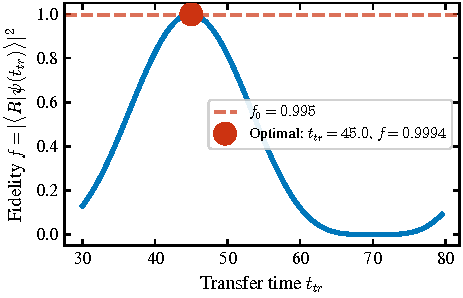
\includegraphics[width=\linewidth]{fig4_fidelity_scan.pdf}
    \figcap{\textbf{Fig.~4} — fidelity vs $t_\mathrm{tr}$; first peak $f=0.999$.}
  \end{block}
  \blockgap

  \begin{block}{3 · Off-centre walls break Rabi}
    Couplings scale exponentially, $J_{LS}/J_{SR}\sim(w/v)^{(\ell_2-\ell_1)/2}$,
    and a three-site chain is capped by
    \[ f_{\max}=\frac{4J_1^2J_2^2}{(J_1^2+J_2^2)^2}. \]
    Fidelity collapses off-centre: $0.637\!\to\!0.061\!\to\!0.004$.
    Shortcut-to-adiabaticity pulses do \emph{not} help — the bottleneck is the
    coupling ratio in the transfer phase, fixed by geometry.
    \centering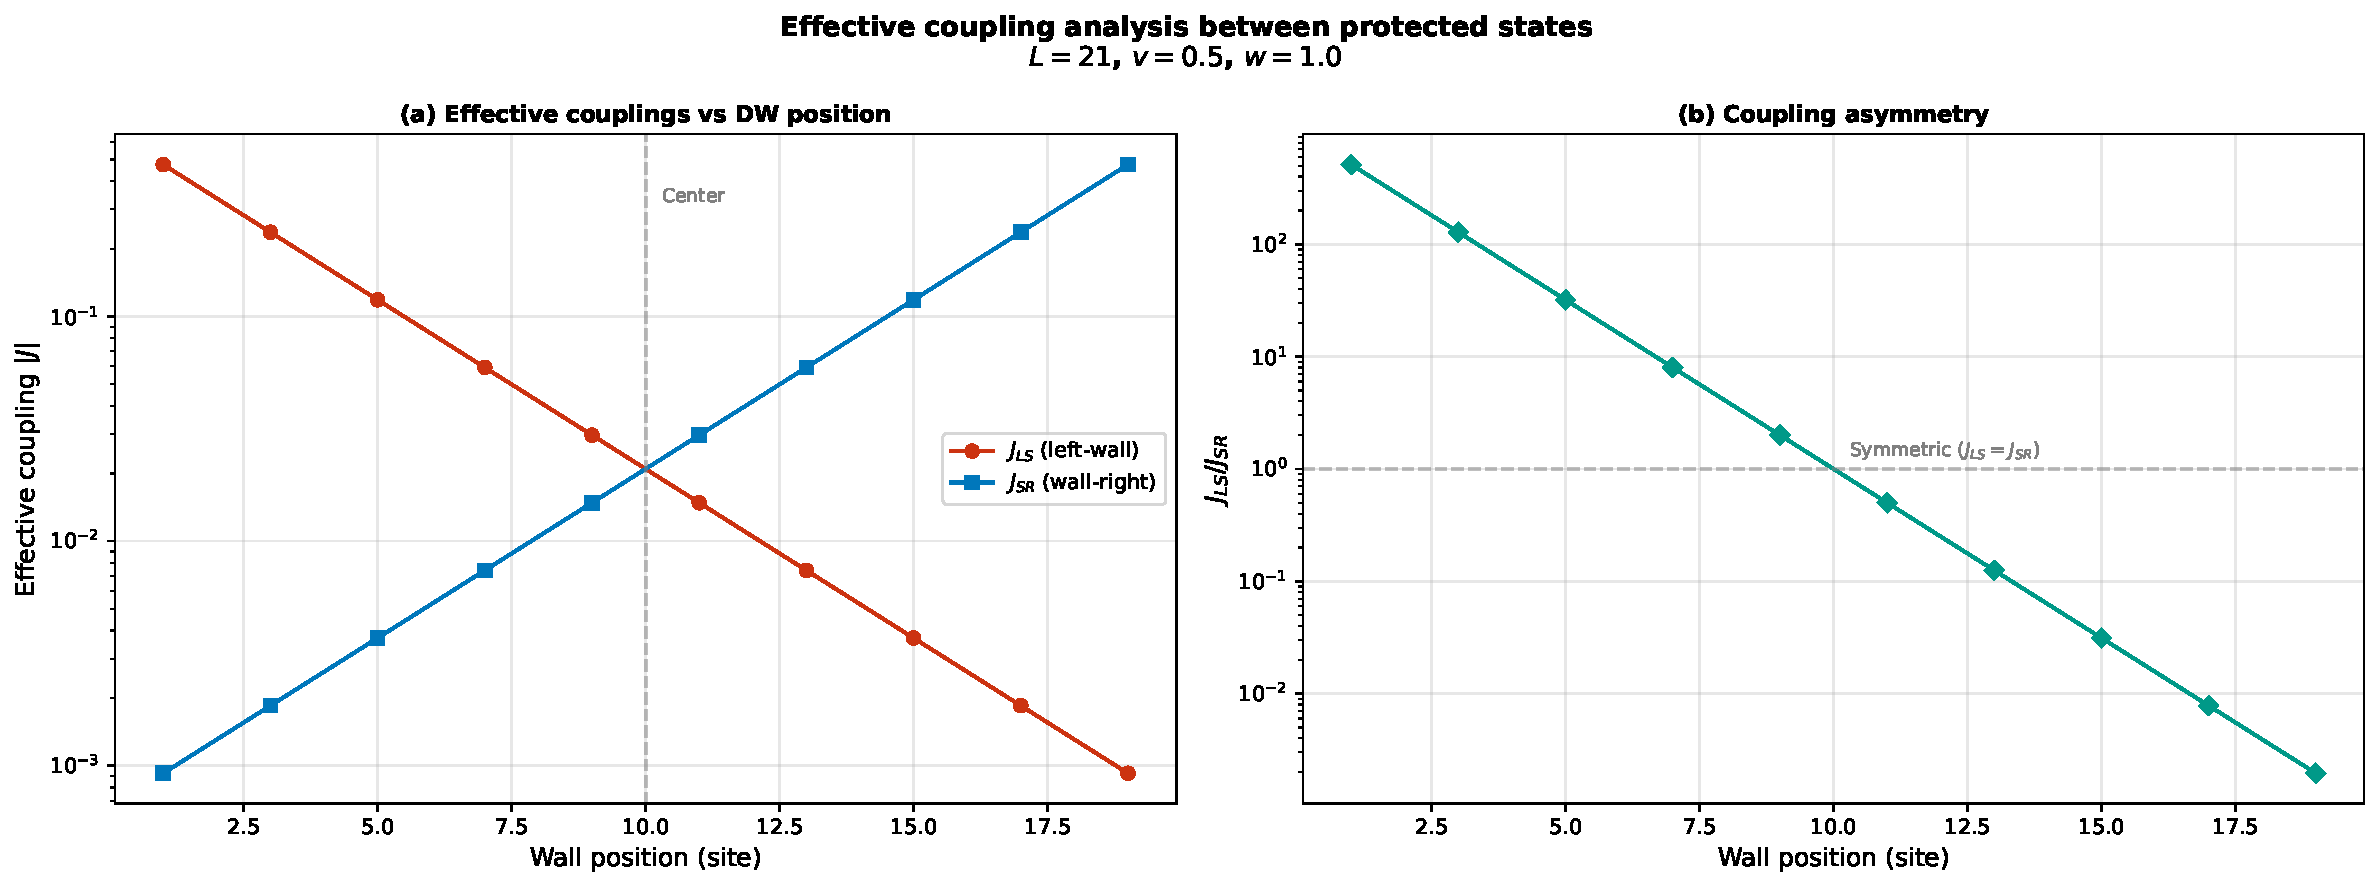
\includegraphics[width=\linewidth]{fig8_effective_coupling.pdf}
    \figcap{\textbf{Fig.~8} — effective couplings vs wall position.}
  \end{block}

\end{minipage}
\end{column}

%---------------- COLUMNA 2 : CTAP (teal) ----------------
\setbeamercolor{block title}{fg=white,bg=tealc}
\setbeamertemplate{itemize item}{\color{tealc}\textbullet}
\begin{column}{0.315\textwidth}
\begin{minipage}[t][\colheight][s]{\linewidth}

  \begin{block}{4 · It's the protocol, not topology}
    The collapse is \textbf{not} a failure of topological protection: the edge
    states stay gapped at every wall position. Give the left and right domains
    \textbf{independent} controls $v_L(t),v_R(t)$. The effective Hamiltonian
    always has a zero-energy \textbf{dark state} with no soliton component:
    \[ \ket{D_0(t)}=\cos\Theta(t)\ket{L}-\sin\Theta(t)\ket{R},\qquad
       \tan\Theta=\frac{J_{LS}}{J_{SR}}. \]
  \end{block}
  \blockgap

  \begin{block}{5 · CTAP dark-state passage}
    Sweeping $\Theta:0\!\to\!\pi/2$ transfers $\ket{L}\!\to\!-\ket{R}$ without
    ever populating $\ket{S}$. Counter-intuitive ordering: $J_{SR}$ fires
    \emph{before} $J_{LS}$; peak amplitudes need not be equal.
    \centering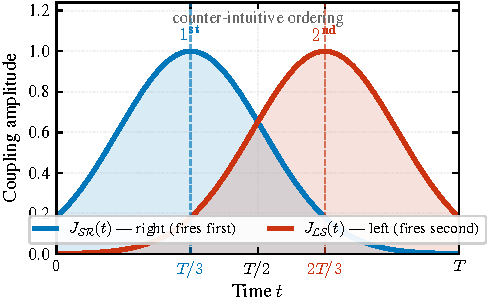
\includegraphics[width=\linewidth]{fig13_ctap_pulses.pdf}
    \figcap{\textbf{Fig.~13} — counter-intuitive pulses; $\ket{S}\approx0$.}
  \end{block}
  \blockgap

  \begin{block}{6 · Full-chain validation ($L=21$)}
    \centering
    \begin{tabular}{cccc}
      \toprule
      $j_\mathrm{DW}$ & Rabi & \textbf{CTAP} & leakage\\
      \midrule
      11 & 0.637 & \textbf{0.9998} & ${<}10^{-7}$\\
      7  & 0.061 & \textbf{0.9999} & ${<}10^{-7}$\\
      5  & 0.004 & \textbf{0.9995} & ${<}10^{-7}$\\
      \bottomrule
    \end{tabular}
    \par\medskip\raggedright
    The $3{\times}3$ reduction is exact to ${<}0.025\%$. The only residual
    infidelity is a removable ceiling $f\le\cos^2\Theta_0$ — not a topological
    bound. Asymmetry is paid in \textbf{time, not fidelity}.
    \centering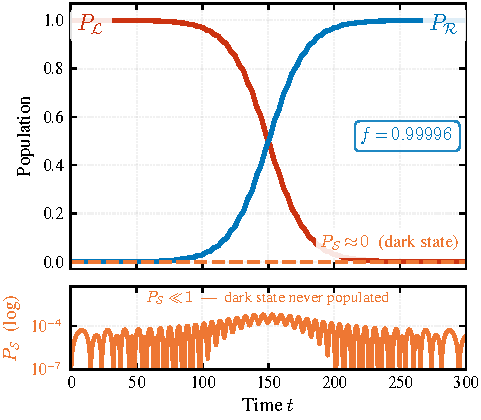
\includegraphics[width=\linewidth]{fig14_ctap_dynamics.pdf}
    \figcap{\textbf{Fig.~14} — Rabi collapses; CTAP holds $f\gtrsim0.99$.}
  \end{block}

\end{minipage}
\end{column}

%---------------- COLUMNA 3 : VELOCIDAD Y ROBUSTEZ (azul) ----------------
\setbeamercolor{block title}{fg=white,bg=ptblue}
\setbeamertemplate{itemize item}{\color{ptblue}\textbullet}
\begin{column}{0.315\textwidth}
\begin{minipage}[t][\colheight][s]{\linewidth}

  \begin{block}{7 · Collective CTAP speed-up}
    Single-wall CTAP is slow ($T$ grows exp.\ with the longest domain).
    Subdividing into $D$ domains shrinks the bottleneck: up to
    $\boldsymbol{\times 13134}$ at $D=4$. A single collective sequence drives
    the $D=4$ chain ($L=45$) with $F=0.998$, NN couplings only.
    \centering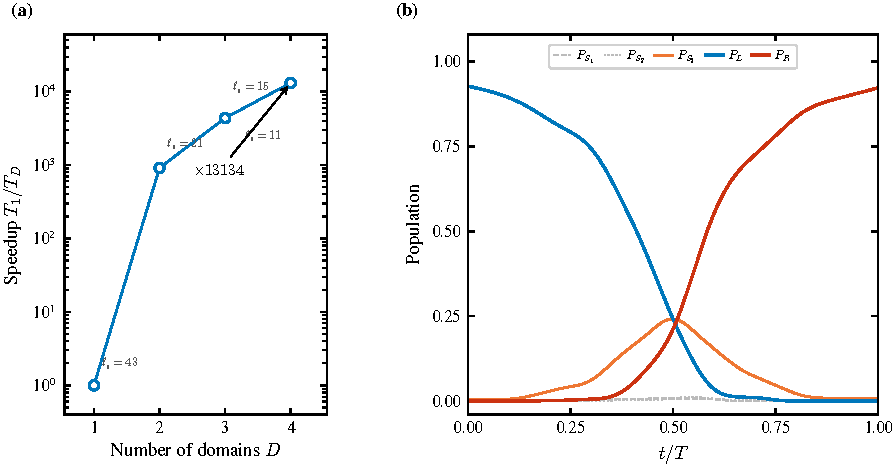
\includegraphics[width=\linewidth]{fig_multidomain_speedup.pdf}
    \figcap{\textbf{Fig.~17} — speed-up and collective transfer.}
  \end{block}
  \blockgap

  \begin{block}{8 · Chiral symmetry sets robustness}
    Off-diagonal disorder respects chiral symmetry: the zero mode stays pinned
    at $E=0$ to $\sim10^{-16}$ and CTAP fidelity stays flat at $\approx0.99$.
    On-site disorder and NNN hoppings break it
    ($\langle|E_0|\rangle\approx0.95\,\kappa$); on-site disorder drives
    $f\to0.30$ at $\sigma=0.20$. CTAP (NN) \textbf{inherits} the protection;
    the CD protocol (NNN) \textbf{forfeits} it. CTAP is also ${\sim}8\times$
    more tolerant to wall misplacement.
    \centering
\includegraphics[width=\linewidth]{fig_robustness_chiral.pdf}
    \figcap{\textbf{Fig.~18} — zero-mode energy and fidelity under disorder.}
  \end{block}
  \blockgap

  \begin{block}{9 · Conclusions}
    \begin{itemize}
      \item Domain-wall transfer reproduced: $f=0.999$ (symmetric).
      \item Static Rabi fails off-centre — a protocol artifact, not a topological limit.
      \item CTAP recovers $f>0.999$ at any wall position; leakage $<10^{-7}$.
      \item Collective multidomain CTAP: $F=0.998$, ${>}4$ orders speed-up.
      \item \textbf{The control protocol — not topology alone — decides robustness.}
      \item Two-wall transfer needs straddling CTAP (even-parity constraint).
    \end{itemize}
  \end{block}

\end{minipage}
\end{column}
\end{columns}

\vspace{0.4cm}

%==================== PIE: REFERENCIAS + QR ====================
\begin{beamercolorbox}[wd=\textwidth,sep=16pt,rounded=true]{footer}
  \begin{minipage}[c]{0.80\textwidth}
    {\small\textbf{References}\quad
    [9] Zurita, Creffield, Platero, \emph{Quantum} \textbf{7}, 1043 (2023).\quad
    [13] Romero, Chen, Platero, Ban, \emph{Phys.\ Rev.\ Applied} \textbf{21}, 034033 (2024).\quad
    [14] Greentree \emph{et al.}, \emph{Phys.\ Rev.\ B} \textbf{70}, 235317 (2004).\quad
    [6] Su, Schrieffer, Heeger, \emph{PRL} \textbf{42}, 1698 (1979).}
    \par\vspace{6pt}
    {\small Acknowledgments: [añadir financiación / grupo]}
  \end{minipage}\hfill
  \begin{minipage}[c]{0.17\textwidth}
    \centering
    \colorbox{white}{\color{black}\qrcode[height=2.8cm]{https://github.com/miguelgarciamier/Quantum-control-for-quantum-information-transfer-mediated-by-topological-edge-states}}\\[4pt]
    {\small Code \& data}
  \end{minipage}
\end{beamercolorbox}

\end{frame}
\end{document}